\hypertarget{introduction}{%
\section{Introduction}\label{introduction}}

Lorem ipsum dolor sit amet, consectetur adipiscing elit. Fusce eu
porttitor purus, ac vestibulum lacus. Donec id mattis dolor. Quisque in
urna et nibh dignissim pulvinar et eget leo. Integer tellus massa,
tincidunt a imperdiet eget, consectetur convallis urna. Nunc laoreet
urna quis massa ullamcorper, quis viverra odio consectetur. Nullam
sodales sed odio non pretium. Cras purus erat, sagittis ac tempus vel,
euismod non leo. Morbi id turpis consequat, laoreet nisl at, iaculis
libero. Nullam eget arcu nec lectus accumsan rutrum. Nunc facilisis, leo
id efficitur eleifend, urna purus tempor nunc, a malesuada lorem ex vel
metus. In ornare imperdiet lorem vitae pretium. Ut sed massa quis metus
sagittis dignissim ac quis orci. Aenean nec blandit tellus, ac tincidunt
tellus. Sed eleifend, ex eu ultrices mollis, ligula augue pulvinar
magna, in tincidunt tortor sem ut augue. Mauris feugiat volutpat elit,
at eleifend eros maximus vitae.

Maecenas vestibulum tempus tellus, eu accumsan justo vulputate quis.
Suspendisse auctor turpis ac dui imperdiet ultrices vitae sit amet nisl.
Fusce vehicula erat id dignissim commodo. Suspendisse iaculis nisl at
dignissim egestas. Sed vestibulum turpis blandit interdum ultricies. In
hac habitasse platea dictumst. Duis at fringilla ante. Donec feugiat
nisi enim, nec eleifend sem bibendum elementum. Pellentesque habitant
morbi tristique senectus et netus et malesuada fames ac turpis egestas.
Praesent efficitur, ligula sed ornare venenatis, mi ligula facilisis
sapien, non pulvinar lacus turpis et lectus. Class aptent taciti
sociosqu ad litora torquent per conubia nostra, per inceptos himenaeos.
Cras ex nunc, faucibus vel scelerisque id, volutpat non ligula. Cras ac
cursus dolor, id scelerisque nibh. Nullam at finibus neque. Aenean
vulputate semper nisl non posuere. Mauris varius mi eget magna malesuada
vulputate.

\hypertarget{methods}{%
\section{Methods}\label{methods}}

\hypertarget{citations}{%
\subsection{Citations}\label{citations}}

Cite literature using \cite{tikhonov1977}. The keys correspond to your
bib file.

\hypertarget{figures}{%
\subsection{Figures}\label{figures}}

Figures can be includes using the standard markdown format. Here is an
example.

\begin{figure}
\centering
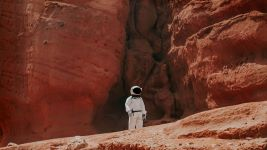
\includegraphics{figures/mars.jpg}
\caption{Insert figure caption here.}
\end{figure}

\hypertarget{more-methods}{%
\subsection{More methods}\label{more-methods}}

Maecenas vestibulum tempus tellus, eu accumsan justo vulputate quis.
Suspendisse auctor turpis ac dui imperdiet ultrices vitae sit amet nisl.
Fusce vehicula erat id dignissim commodo. Suspendisse iaculis nisl at
dignissim egestas. Sed vestibulum turpis blandit interdum ultricies. In
hac habitasse platea dictumst. Duis at fringilla ante. Donec feugiat
nisi enim, nec eleifend sem bibendum elementum. Pellentesque habitant
morbi tristique senectus et netus et malesuada fames ac turpis egestas.
Praesent efficitur, ligula sed ornare venenatis, mi ligula facilisis
sapien, non pulvinar lacus turpis et lectus. Class aptent taciti
sociosqu ad litora torquent per conubia nostra, per inceptos himenaeos.
Cras ex nunc, faucibus vel scelerisque id, volutpat non ligula. Cras ac
cursus dolor, id scelerisque nibh. Nullam at finibus neque. Aenean
vulputate semper nisl non posuere. Mauris varius mi eget magna malesuada
vulputate.

\hypertarget{results}{%
\section{Results}\label{results}}

\hypertarget{result-1}{%
\subsection{Result 1}\label{result-1}}

Proin placerat cursus nisi nec commodo. Nunc ornare mollis nulla nec
varius. Vestibulum dapibus lacus erat, eget mattis tortor hendrerit ut.
Aliquam rhoncus tempus dapibus. Sed in purus nulla. Curabitur at metus
purus. Donec commodo quis est ac molestie. Quisque id elementum ante.
Fusce suscipit massa quis orci scelerisque aliquam. Proin mattis eget
nibh in lobortis. Integer ut mollis odio, nec posuere leo. Nullam purus
mi, hendrerit at nulla id, lobortis vulputate quam.

\begin{figure}
\centering
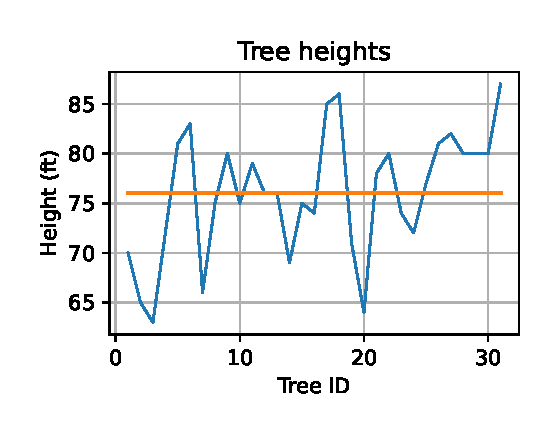
\includegraphics{figures/tree-heights.eps}
\caption{Tree heights for the different trees, and mean tree height.}
\end{figure}

\hypertarget{result-2}{%
\subsection{Result 2}\label{result-2}}

Duis ex sem, vulputate eget interdum et, interdum a nisl. Sed non
egestas augue. Pellentesque auctor velit at viverra tempus. Aliquam vel
orci ullamcorper, molestie leo a, mollis erat. Quisque rutrum sapien eu
volutpat commodo. Cras augue dolor, lacinia auctor viverra ut, bibendum
venenatis purus. Donec quis eros ac nunc auctor varius. Phasellus
laoreet scelerisque odio id mollis. Proin ornare quam ut metus rutrum
tincidunt. Praesent congue sagittis consectetur. Proin sapien nulla,
lacinia nec scelerisque eget, interdum vel enim. Aliquam erat volutpat.
Sed varius dictum orci.

\hypertarget{conclusions}{%
\section{Conclusions}\label{conclusions}}

Donec ac massa eget eros hendrerit sagittis ut eu dolor. Nulla venenatis
finibus est, eget elementum odio ornare ac. Vestibulum in enim mi.
Phasellus nec pulvinar metus. Aenean et tempus augue, id accumsan ipsum.
Duis tempus, velit sit amet accumsan egestas, eros metus aliquam urna,
id accumsan ligula ante vel mauris. Cras feugiat leo eget erat tempus
accumsan. Nullam ut justo urna. Proin vel diam magna. Cras sed
pellentesque orci. Vestibulum scelerisque nulla feugiat purus pretium,
id elementum libero tempus. Orci varius natoque penatibus et magnis dis
parturient montes, nascetur ridiculus mus.
